\documentclass{tufte-handout}

\title{Backprojection}

\author[Jan Gaura]{Jan Gaura}

%\date{28 March 2010} % without \date command, current date is supplied

%\geometry{showframe} % display margins for debugging page layout

\usepackage{graphicx} % allow embedded images
  \setkeys{Gin}{width=\linewidth,totalheight=\textheight,keepaspectratio}
  \graphicspath{{graphics/}} % set of paths to search for images
\usepackage{amsmath}  % extended mathematics
\usepackage{booktabs} % book-quality tables
\usepackage{units}    % non-stacked fractions and better unit spacing
\usepackage{multicol} % multiple column layout facilities
\usepackage{lipsum}   % filler text
\usepackage{fancyvrb} % extended verbatim environments
  \fvset{fontsize=\normalsize}% default font size for fancy-verbatim environments

% Standardize command font styles and environments
\newcommand{\doccmd}[1]{\texttt{\textbackslash#1}}% command name -- adds backslash automatically
\newcommand{\docopt}[1]{\ensuremath{\langle}\textrm{\textit{#1}}\ensuremath{\rangle}}% optional command argument
\newcommand{\docarg}[1]{\textrm{\textit{#1}}}% (required) command argument
\newcommand{\docenv}[1]{\textsf{#1}}% environment name
\newcommand{\docpkg}[1]{\texttt{#1}}% package name
\newcommand{\doccls}[1]{\texttt{#1}}% document class name
\newcommand{\docclsopt}[1]{\texttt{#1}}% document class option name
\newenvironment{docspec}{\begin{quote}\noindent}{\end{quote}}% command specification environment

\begin{document}

\maketitle% this prints the handout title, author, and date

\begin{figure*}[h]
  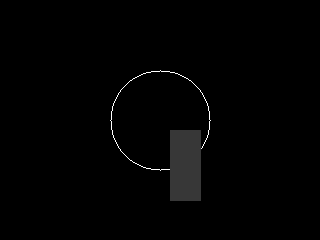
\includegraphics[width=0.3\linewidth]{images/input.png}
  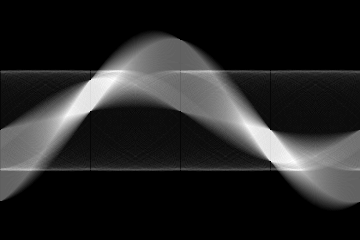
\includegraphics[width=0.337\linewidth]{images/sinogram.png}
  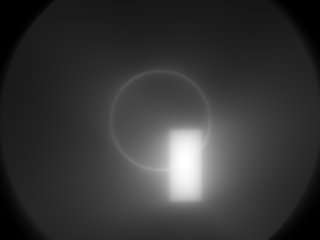
\includegraphics[width=0.3\linewidth]{images/backprojected.png}
  \caption{\emph{Left:} Input image, \emph{middle:} sinogram, \emph{right:} backprojected image.
  %\emph{Notice that this figure takes up the full page width.}
  }%
  \label{fig:title}%
\end{figure*}

%\begin{abstract}
%\noindent
%This document describes the Tufte handout \LaTeX\ document style.
%It also provides examples and comments on the style's use.
%Only a brief overview is presented here;
%for a complete reference, see the sample book.
%\end{abstract}

%\printclassoptions

The goal of this exercise is to implement projection and backprojection algorithms
to reconstruct an image from a finite number of projections\cite{wiki-tomographic-reconstruction}.
A notable use of this technique is the reconstruction of computer tomography.

\section{Projection}

To complete our task, we create an image as shown in Fig.~\ref{fig:title} (\emph{left})
(but you can create also other image to your liking).

What we do next, is to create projections of the input image in given number of angles
($\langle 0, 180 \rangle$, with step of 1).
By projection we mean the sum of image pixel brightnesses along a line.\footnote{Don't
forget that such sum can result in values greater than 255 and you have to set the type
of \texttt{cv::Mat} accordingly.}
This projection creates a vector.
Projecting the input image in different angles would be tedious,
so we can use a little trick. We rotate the input image by the given angle and project
the rotated image along the $x$-axis.
In this way, we can store each projection as a vector and set of all projections
as an image (see Fig.~\ref{fig:title} (\emph{middle})). Such image is called sinogram.


\section{Backprojection}

From the set of vectors with each projection, we reconstruct the input image.
First, we take each projection and reconstruct an image so that we copy the projection
vector to each column of reconstructed projection image. Then we rotate this image
by the angle the projection was taken from. Then we stack all such reconstructed projection
images and sum values in each pixel to obtain the final image
(see Fig.~\ref{fig:title} (\emph{right}) for the final result.\marginnote{Note the clearly
visible circle in the backprojected image.}


\bibliography{backprojection}
\bibliographystyle{plainnat}



\end{document}
